%%%%%%%%                       01 - Motivation                      %%%%%%%%
%---------------------------------------------------------------------------
% When presenting, the beginning is what matters most. 
% To attract attention at the beginning of a public speech, it is advisable to: tell a statistic; ask a question (more like a rhetorical question for the state final exam).

% HEROUT, Adam. Prezentování. Herout.net: Poznámky učitele, kouče, čtenáře. [online]. [cit. 2021-9-15]. Available at: https://www.herout.net/blog/category/prezentovani/
%---------------------------------------------------------------------------

% - Introduce the audience to the topic of your thesis.
% - Tell a little about the situation before you started your work and what were the reasons for developing it.
% - It is best to explain the motivation using a scheme. If you must use bullet points, make them super-short so you don't read them, but they only form the skeleton of the message.

% From this part of the presentation, the audience must get brief and concise answers to the questions:
%  A) Why your work should matter? What is it good for?
%  B) What is the aim of the work? What should be the result?

% Resist the temptation to say banalities and common knowledge.+
% "We live in an age of mobile computing where everyone has a mobile phone in their pocket" - is an empty and stupid statement, don't say anything like that, nobody cares.

\begin{frame}
  \frametitle{Motivation}
  \begin{columns}
    \column{0.4\textwidth}
    \begin{itemize}
        \item \emph{Inputs} or state \emph{before}
        \item What should be the~\emph{outputs}
        \item \emph{No} or \emph{brief} bullets!
        \item Desirable: A scheme with inputs and outputs
    \end{itemize}
     
    \column{0.6\textwidth}
    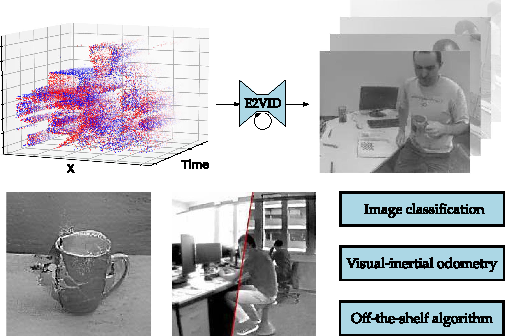
\includegraphics[width=\textwidth]{img/template-Teaser.pdf}
  \end{columns}
\end{frame}


%%%%%%%%                       02 - Objectives                      %%%%%%%%
%---------------------------------------------------------------------------
% Briefly state the objectives of your thesis.
% Up to 3 bullets/sentences with main objectives are suitable.

% Sometimes, the motivation is identical to the formulation of goals. Don't force yourself into two slides when the idea is best conveyed in one...

% Formulate what the goal is:
%  - How do you know a successful outcome?
%  - What are the results?
%  - What are the characteristics of a successful result?
%  - Where can it be used?

% Better without using bullets:
%  - have a good enough picture to comment on in your own words 
%  - a figure is the best visual message and you deliver the verbal message with your mouth

% It is useless to make generic and general statements "The solution should be fast, reliable and robust" - these are general requirements for anything, and the informational value of the message is ZERO - it is just a waste of time and intellect.
% Be specific: What specific features should your solution have, what "robust" means specifically, what "reliable" means precisely?

\begin{frame}
  \frametitle{Objectives of the Thesis}
  \begin{columns}
    \column{0.4\textwidth}
    \begin{itemize}
        \item \emph{Input}
        \item \emph{Output}
        \item Desirable \emph{properties}
        \item Uses \& applications
    \end{itemize}
     
    \column{0.6\textwidth}
        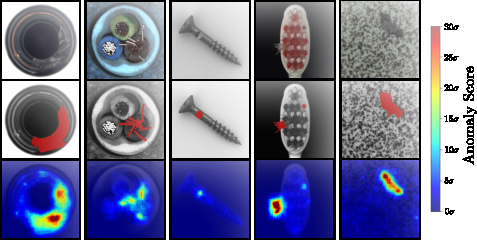
\includegraphics[width=\textwidth]{img/template-Goal.pdf}
  \end{columns}
\end{frame}


%%%%%%%%                      03 - Information                      %%%%%%%%
%---------------------------------------------------------------------------
% The purpose of the defence is to report on the project's status, not to hold a lecture on the given topic. Talk about what you have done and what your results are. Keep formal terms on your slides, be precise, define and refer.

% The presentation need not and, in fact, should not include:
% -- Explanation of algorithms used, etc. That belongs in a lecture about the topic. In your project presentation, it is typically enough just to list the used algorithms by name. Unknown algorithms can be explained a bit to clarify what they are, but don't explain them in detail. The goal is not for your audience to completely understand the algorithm and to be able to program it but to give them an idea of what you are working on and how you are doing it.
% -- Details of your system design. Again, your audience is not going to hack your system; they don't need detailed class structure, function names, file names, data formats, etc. Provide these things only to the extent that it helps the audience understand what you're are working on and how you are succeeding in it.

% HEROUT, Adam. Prezentování. Herout.net: Poznámky učitele, kouče, čtenáře. [online]. [cit. 2021-9-15]. Available at: https://www.herout.net/blog/category/prezentovani/
%---------------------------------------------------------------------------

% - Indicate what interesting problems you have solved in your thesis.
% - It should show that it is a thesis -- not just another project for a course -- so there is something non-trivial, interesting, and useful.
% - Rather have two or three slides that you show/explain in 20 seconds than trying to cram everything onto one slide.
% - It is good to put visual information on the slides: formulas, schemes, pictures, diagrams. Verbal information can be conveyed through your mouth. It is perfectly useless and annoying to have the same thing you are going to say in bullets on a slide.
% - The title of the slide, "Essential Information About the Solution", is very generic. In your actual slides, it would be much better to use a specific title on each of the slides, for example, "Neural Network Scheme for Big Nose Detection", "Design of an Infinite Automata", "Collected Dataset", etc.

\begin{frame}
  \frametitle{Essential Information About the Solution}
  \centering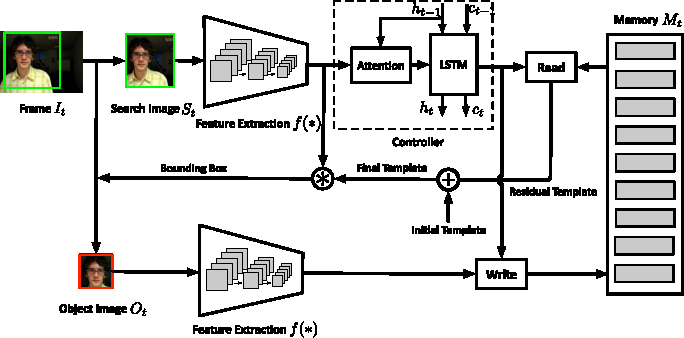
\includegraphics[width=0.8\textwidth]{img/template-Schema.pdf}
  \begin{equation}
      \mathbf{a}_t = \sum_{i=1}^{L}\alpha_{t,i}\mathbf{f}_{t,i}^{*}
  \end{equation}
  where $\alpha_{t,i}$ computes the \emph{softmax}:
  \begin{align}
      \alpha_{t,i} &= \frac{\exp(r_{t,i})}{\sum_{k=1}{L}\exp(r_{t,k})} 
      \\
      r_{t,i} &= W^a \tanh\left( W^h \mathbf{h}_{t-1} + W^f\mathbf{f}_{t,i}^{*} + b \right)
  \end{align}
\end{frame}

\begin{frame}\frametitle{Essential Information About the Solution}
  \makebox[\linewidth]{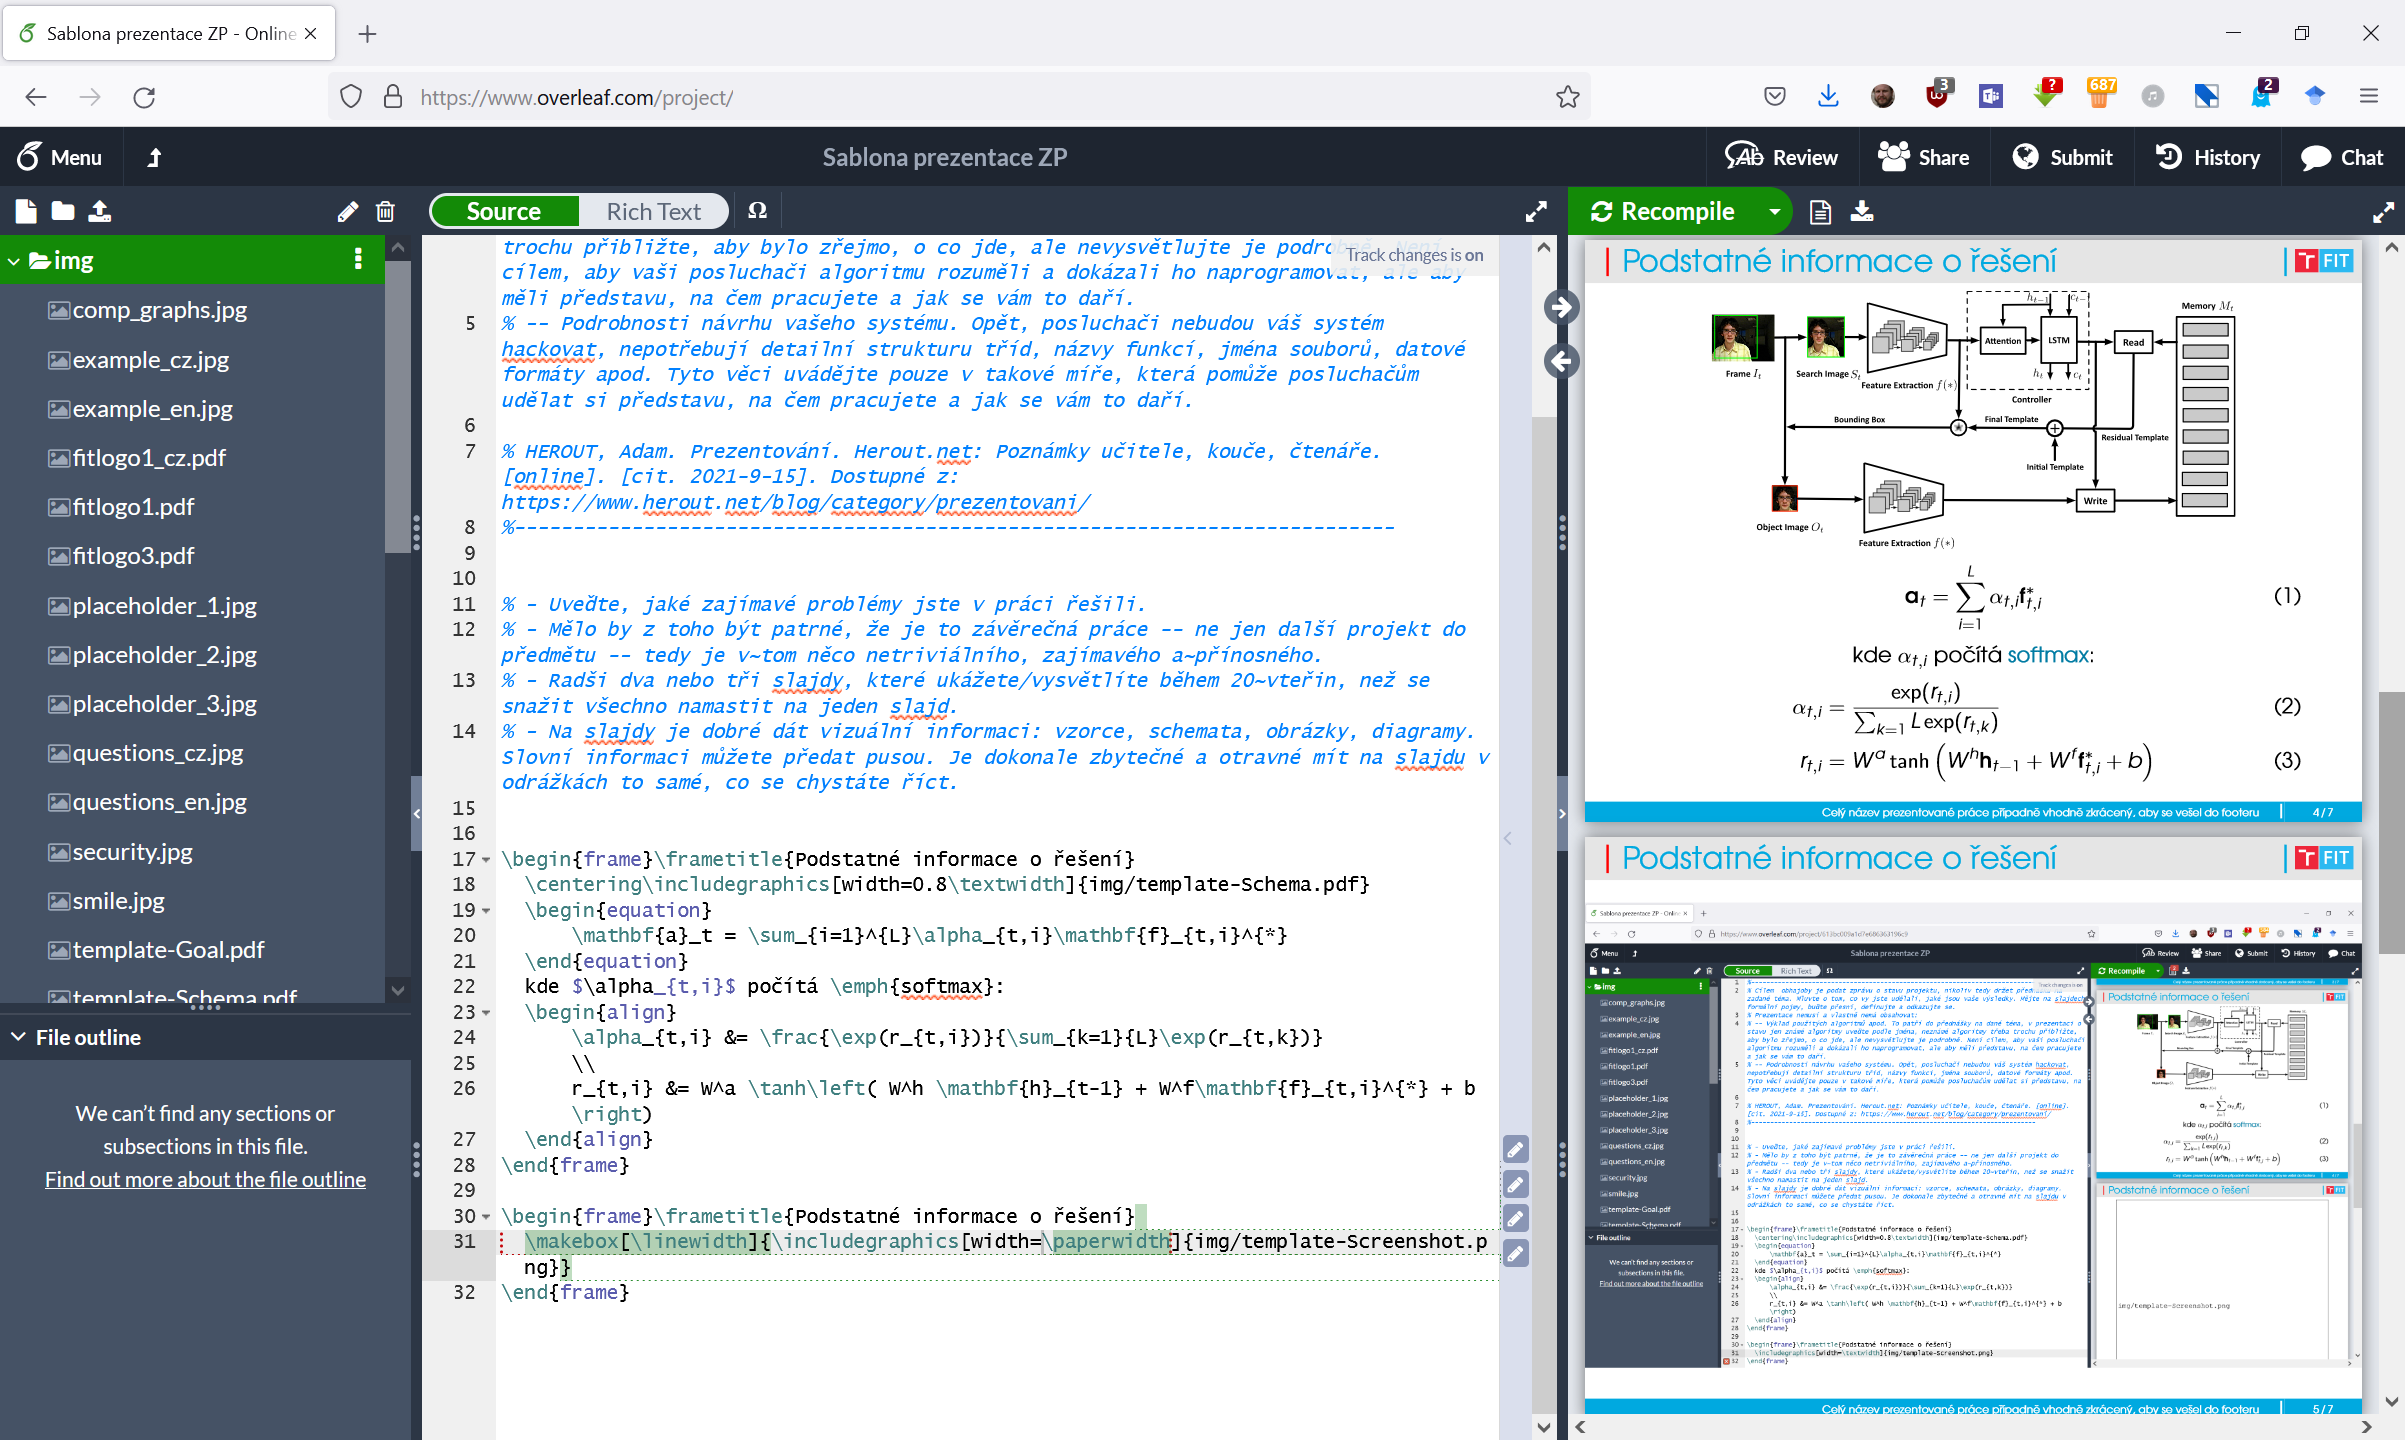
\includegraphics[width=\paperwidth]{img/template-Screenshot.png}}
\end{frame}


%%%%%%%%                        04 - Results                        %%%%%%%%
%---------------------------------------------------------------------------
% Summarise what results in you have achieved.
% Indicate how the functionality and correctness of the solution have been evaluated.
% Be specific: instead of "The application has been tested", say by whom and how it has been tested, and what the test results were.
% Instead of "The detector success rate is very good", say "The detector success rate is 93% mAP", or even better, show a table with a comparison against alternative solutions.
% If the evaluation consisted of two or three parts, splitting the content into two or three slides may be appropriate. When presenting, however, care should be taken to ensure that the time devoted to each slide is adequately short and that there is no time overrun.

\begin{frame}
  \frametitle{Experimental Results}
  \begin{columns}
  \column{0.4\textwidth}
    \begin{itemize}
      \item What has been \emph{done}
      \item Created dataset: \emph{105\,thousand} records
      \item Success Rate: \emph{103\,\%}
    \end{itemize}
    
  \column{0.6\textwidth}
    \centering
    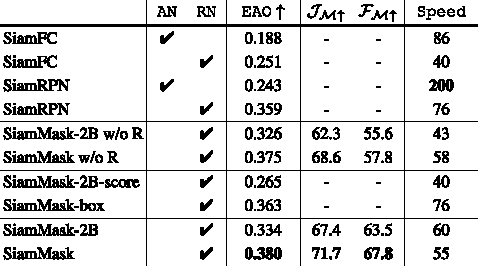
\includegraphics[width=0.8\textwidth]{img/template-ResultsTable.pdf}
    
    \bigskip
    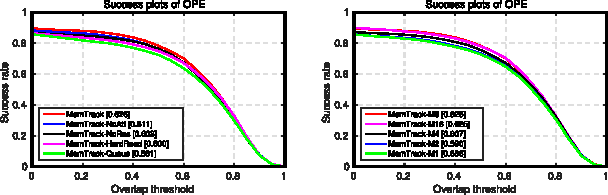
\includegraphics[width=\textwidth]{img/template-ResultsPlot.pdf}
    
  \end{columns}
\end{frame}


%%%%%%%%                        05 - Thanks                         %%%%%%%%
%---------------------------------------------------------------------------
% This slide should contain either one large or several smaller images arranged appropriately.
% Choose the best thing you want to show off - the committee will look at this slide the longest of all the slides.
% For this slide, thank the committee for attention (not necessarily by a huge text over the whole slide), and the committee will then have space to view the images as they listen to the reviews.
%---------------------------------------------------------------------------

% What is said at the end of the presentation is what the audience will consider when making subsequent decisions.

% HEROUT, Adam. Prezentování. Herout.net: Poznámky učitele, kouče, čtenáře. [online]. [cit. 2021-9-15]. Available at: https://www.herout.net/blog/category/prezentovani/
%---------------------------------------------------------------------------

\begin{frame}
  \frametitle{Thank You for Your Attention!}
  \centering
  \makebox[\textwidth]{
    \begin{tikzpicture}
      \node (screenshot) 
         {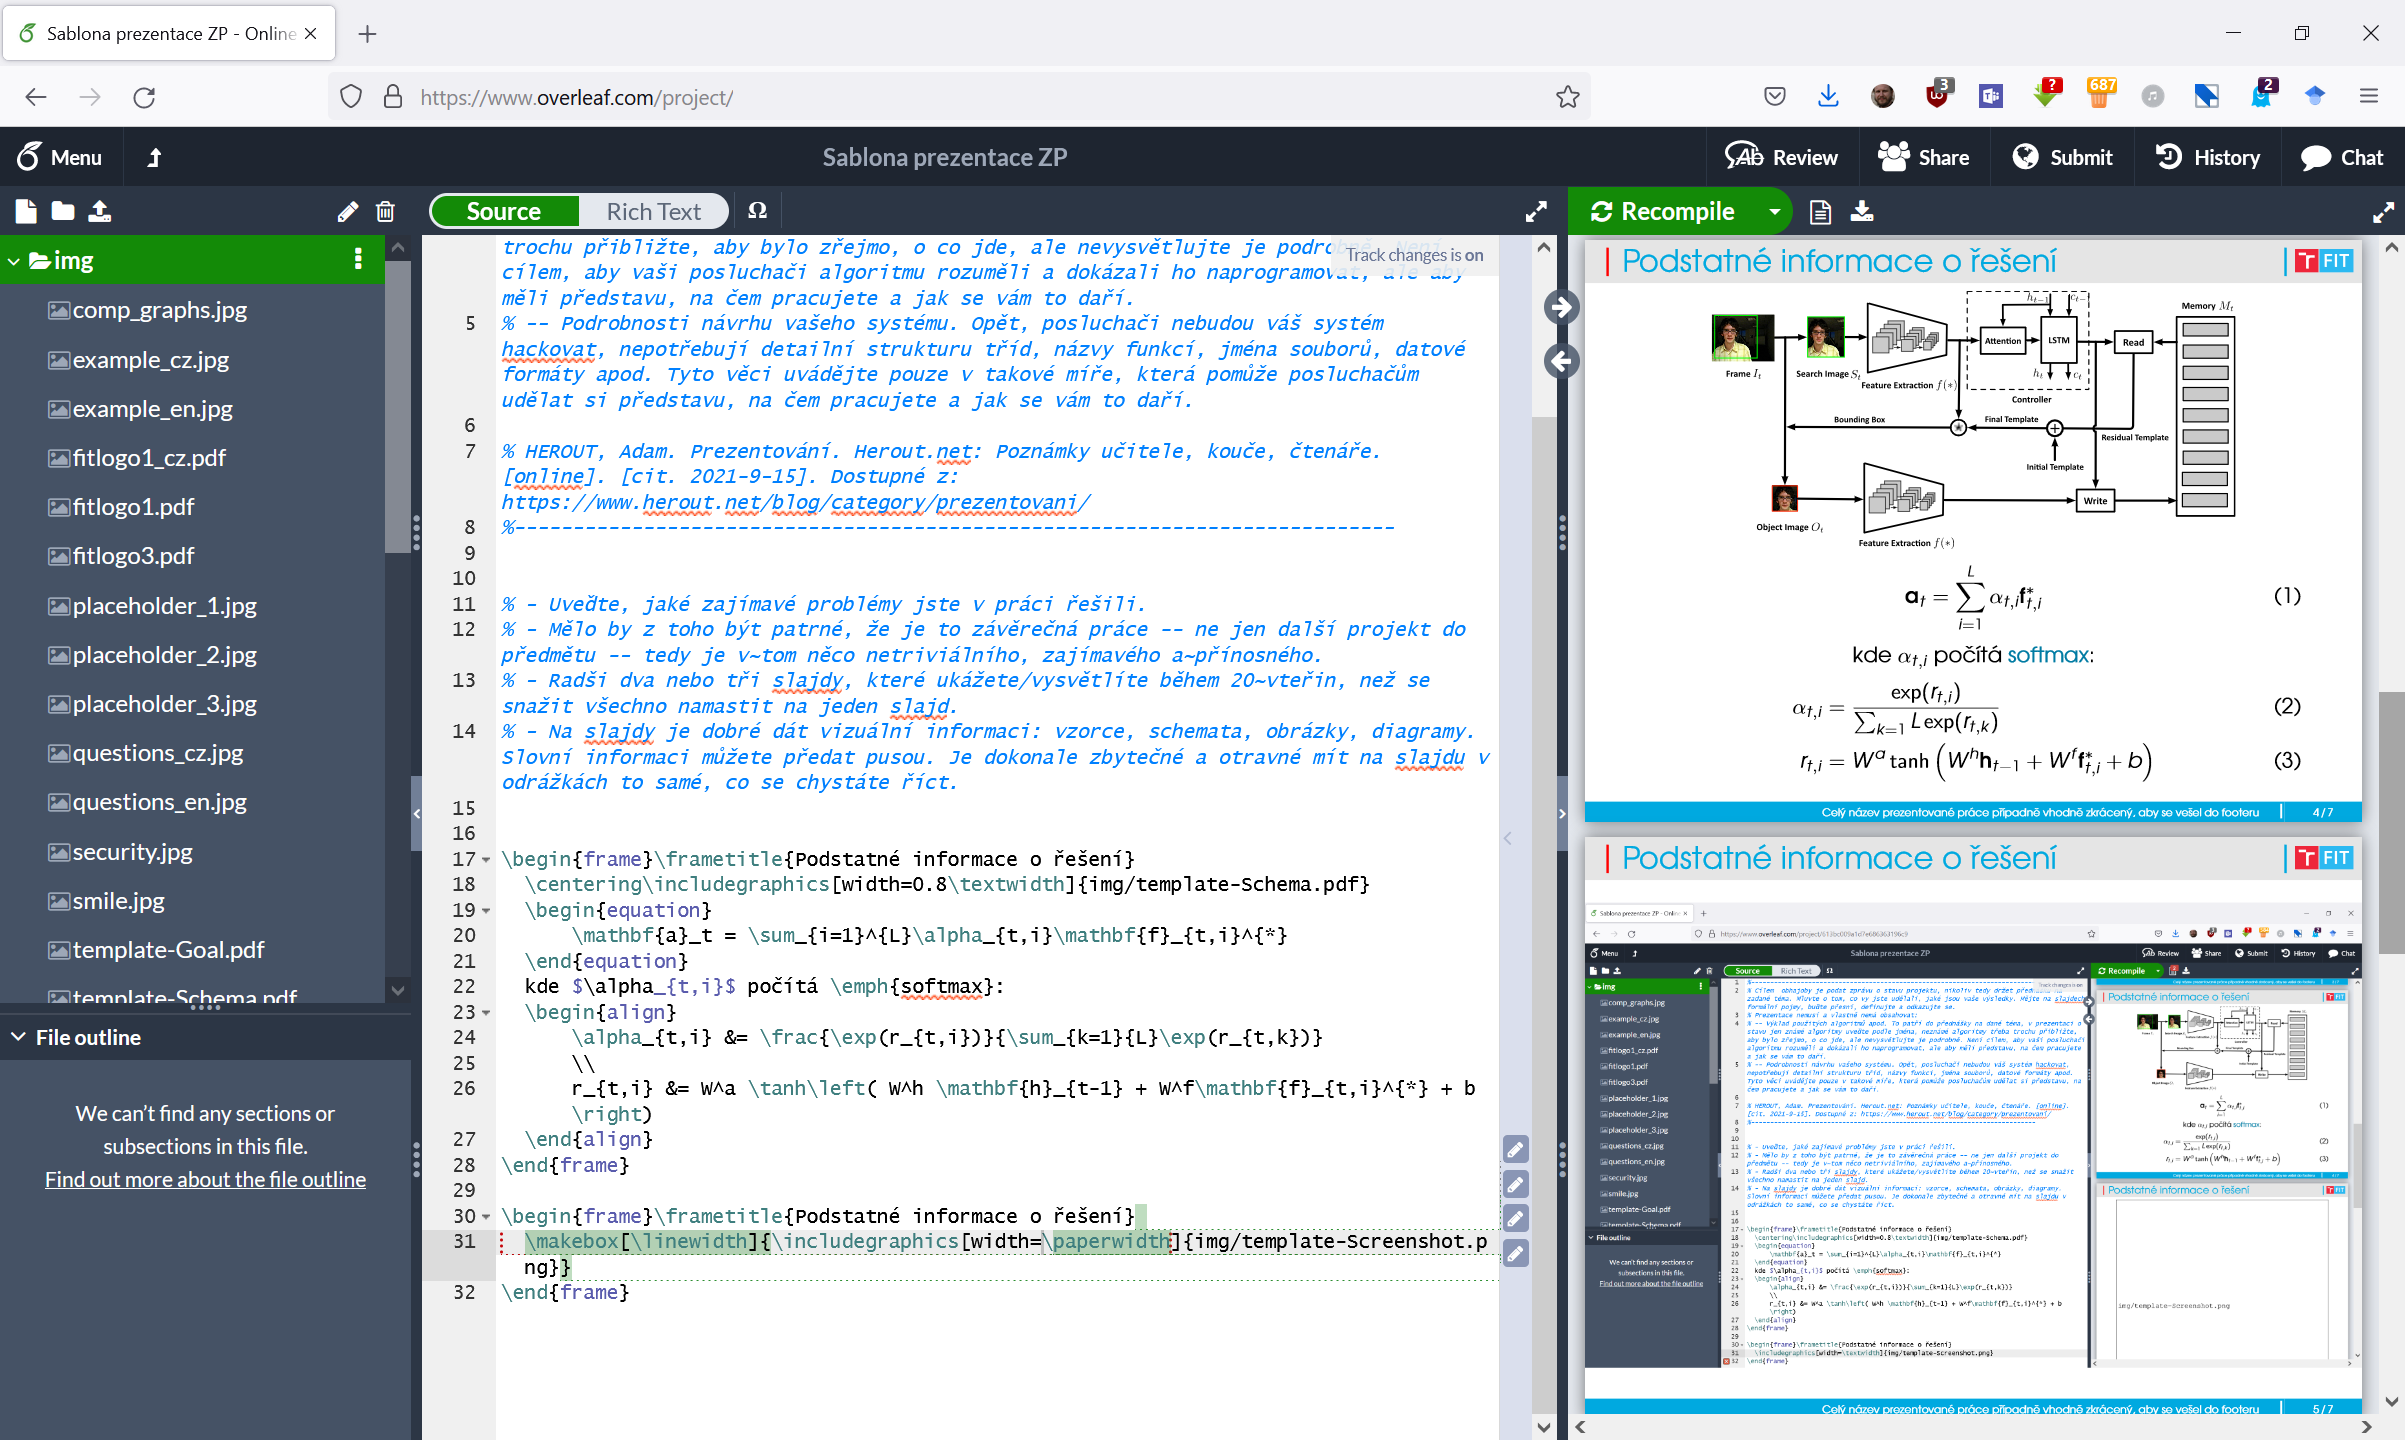
\includegraphics[width=0.6\paperwidth]{img/template-Screenshot.png}};
      \node (schema) at (screenshot.south east) [xshift=5em] [yshift=2.5ex]
         {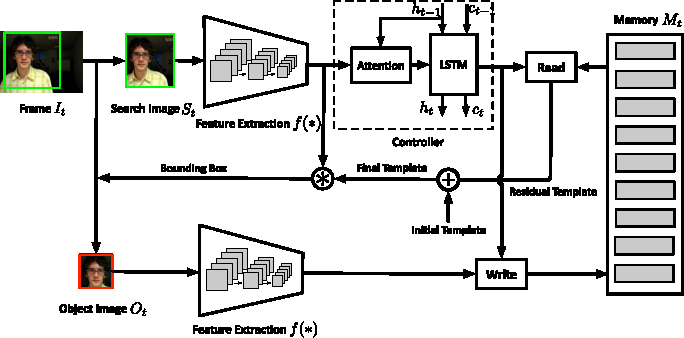
\includegraphics[width=0.45\paperwidth]{img/template-Schema.pdf}};
      \node (goal) at (screenshot.north east) [xshift=4em] [yshift=2ex]
         {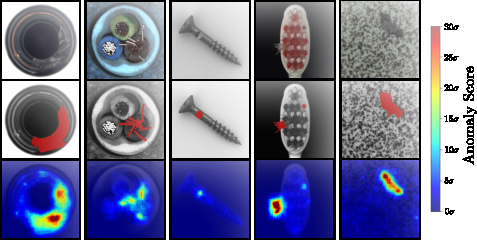
\includegraphics[width=0.5\paperwidth]{img/template-Goal.pdf}};
    \end{tikzpicture}
  }
\end{frame}


%%%%%%%%                       06 - Questions                       %%%%%%%%
%---------------------------------------------------------------------------
% At the State final examination:
%   1) The student presents his/her thesis, ends with "Thank you for your attention!"
%   2) The commission chairman organises what happens next: an extract from the reviews is read.
%   3) The student will answer the questions that the opponent has written in his/her review.
%   4) The student answers questions that come up in the room: from the committee members, but also from the guests.

% For point 3) above, it is helpful to have prepared slides:
%   A) They show the verbatim text of the opponent's question. The student reads it so that everyone knows it, and then answers it.
%   B) They will include visual aids to the answer.
%       a) Some answers to questions do not need visual support: the student simply says the answer, and everything is clear.
%       b) For other answers, it is wise to have a picture, a table, a graph, something that clearly shows the answer.

% The opponent's questions are not meant to be "topics for a lecture". If it can be answered in one sentence, it's better than fumbling around.
% Visual aids often help to answer succinctly, "The figure shows how I solve problem X." And that's it...

% If no visual information is needed for the questions, it is helpful to have them as bullets on a single slide.
% If there is more than one question and there are figures or graphs, it is advisable to have one slide for each question - the text of the question at the top, the visual material below.

\appendix{}
\begin{frame}
  \frametitle{Opponent's Questions}
  \begin{itemize}
    \item If there are multiple questions, more slides can be made.
    \item This slide should be an attachment that does not count towards the total number of slides.
    \item It is a good idea to transcribe the question here \emph{verbatim}, so that there is no doubt that there is no inaccurate paraphrasing.
  \end{itemize}
  \bigskip
  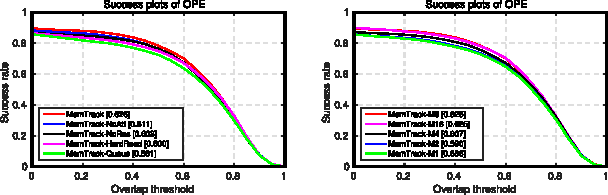
\includegraphics[width=\textwidth]{img/template-ResultsPlot.pdf}
\end{frame}